\begin{figure}
    \centering
        \tikzset{every picture/.style={line width=0.75pt}} %set default line width to 0.75pt        
        
            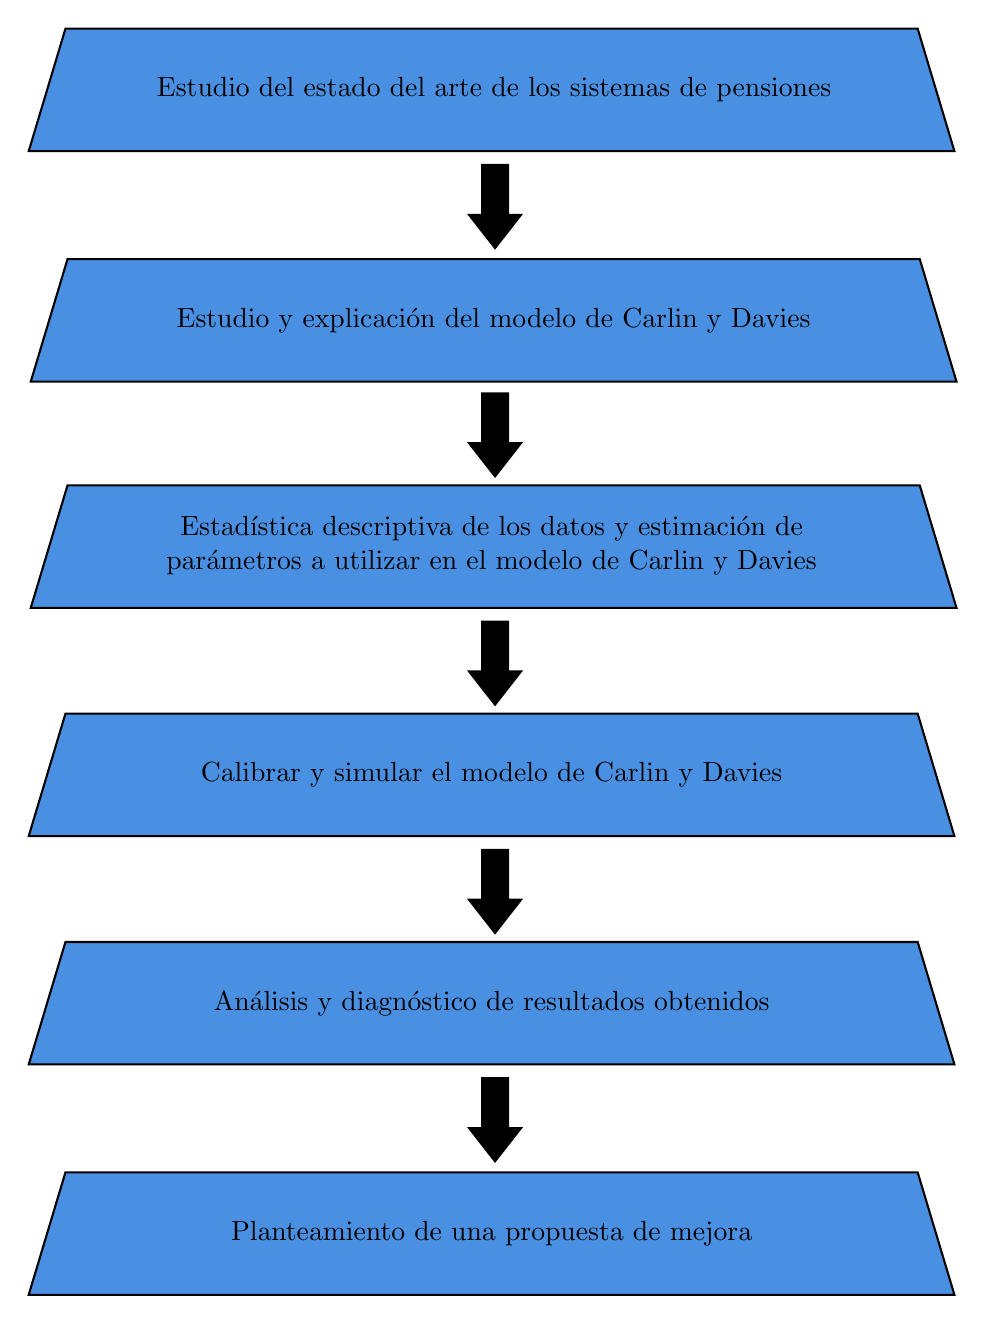
\begin{tikzpicture}[x=0.75pt,y=0.75pt,yscale=-1,xscale=1]
            %uncomment if require: \path (0,847); %set diagram left start at 0, and has height of 847
        
            %Shape: Trapezoid [id:dp16310007281939687] 
            \draw  [fill={rgb, 255:red, 74; green, 144; blue, 226 }  ,fill opacity=1 ] (70.5,70) -- (88.2,11) -- (498.8,11) -- (516.5,70) -- cycle ;
            %Down Arrow [id:dp47868702740650404] 
            \draw  [fill={rgb, 255:red, 0; green, 0; blue, 0 }  ,fill opacity=1 ] (282.67,100.67) -- (288.92,100.67) -- (288.92,76.67) -- (301.42,76.67) -- (301.42,100.67) -- (307.67,100.67) -- (295.17,116.67) -- cycle ;
            %Shape: Trapezoid [id:dp5963598053062951] 
            \draw  [fill={rgb, 255:red, 74; green, 144; blue, 226 }  ,fill opacity=1 ] (71.5,181) -- (89.2,122) -- (499.8,122) -- (517.5,181) -- cycle ;
            %Down Arrow [id:dp3449357365692677] 
            \draw  [fill={rgb, 255:red, 0; green, 0; blue, 0 }  ,fill opacity=1 ] (282.67,210.67) -- (288.92,210.67) -- (288.92,186.67) -- (301.42,186.67) -- (301.42,210.67) -- (307.67,210.67) -- (295.17,226.67) -- cycle ;
            %Shape: Trapezoid [id:dp1505077896190936] 
            \draw  [fill={rgb, 255:red, 74; green, 144; blue, 226 }  ,fill opacity=1 ] (71.5,290) -- (89.2,231) -- (499.8,231) -- (517.5,290) -- cycle ;
            %Down Arrow [id:dp04773390289061186] 
            \draw  [fill={rgb, 255:red, 0; green, 0; blue, 0 }  ,fill opacity=1 ] (282.67,320.67) -- (288.92,320.67) -- (288.92,296.67) -- (301.42,296.67) -- (301.42,320.67) -- (307.67,320.67) -- (295.17,336.67) -- cycle ;
            %Shape: Trapezoid [id:dp4086537842538548] 
            \draw  [fill={rgb, 255:red, 74; green, 144; blue, 226 }  ,fill opacity=1 ] (70.5,400) -- (88.2,341) -- (498.8,341) -- (516.5,400) -- cycle ;
            %Down Arrow [id:dp13371932006774911] 
            \draw  [fill={rgb, 255:red, 0; green, 0; blue, 0 }  ,fill opacity=1 ] (282.67,430.67) -- (288.92,430.67) -- (288.92,406.67) -- (301.42,406.67) -- (301.42,430.67) -- (307.67,430.67) -- (295.17,446.67) -- cycle ;
            %Shape: Trapezoid [id:dp8626602729324185] 
            \draw  [fill={rgb, 255:red, 74; green, 144; blue, 226 }  ,fill opacity=1 ] (70.5,510) -- (88.2,451) -- (498.8,451) -- (516.5,510) -- cycle ;
            %Down Arrow [id:dp24496247527071058] 
            \draw  [fill={rgb, 255:red, 0; green, 0; blue, 0 }  ,fill opacity=1 ] (282.67,540.67) -- (288.92,540.67) -- (288.92,516.67) -- (301.42,516.67) -- (301.42,540.67) -- (307.67,540.67) -- (295.17,556.67) -- cycle ;
            %Shape: Trapezoid [id:dp9556756619131235] 
            \draw  [fill={rgb, 255:red, 74; green, 144; blue, 226 }  ,fill opacity=1 ] (70.5,621) -- (88.2,562) -- (498.8,562) -- (516.5,621) -- cycle ;
            
            % Text Node
            \draw (294.75,40.25) node   [align=left] {Estudio del estado del arte de los sistemas de pensiones};
            % Text Node
            \draw (294.5,151.5) node   [align=left] {Estudio y explicación del modelo de Carlin y Davies};
            
            % Text Node
            \draw (293.5,260) node   [align=left] {\begin{minipage}[lt]{241.96pt}\setlength\topsep{0pt}
            \begin{center}
            Estadística descriptiva de los datos y estimación de parámetros a utilizar en el modelo de Carlin y Davies
            \end{center}\end{minipage}};
            
            % Text Node
            \draw (293.5,370.5) node   [align=left] {Calibrar y simular el modelo de Carlin y Davies};
            % Text Node
            \draw (293.5,480.5) node   [align=left] {Análisis y diagnóstico de resultados obtenidos};
            % Text Node
            \draw (293.5,591.5) node   [align=left] {Planteamiento de una propuesta de mejora};
        
            \end{tikzpicture}

    \caption{Diagrama metodología}
    \label{fig:metodología}
\end{figure}